\section{Факторпространства}

\subsection{Теоретико-множественное отступление}

Факторизация множеств и отображений упрощает сложные структуры, сводя их к более удобным формам. Она широко применяется в топологии, алгебре и других областях для изучения симметрий и инвариантов.

Интуитивно, факторизация группирует элементы множества так, чтобы сосредоточиться на глобальных свойствах, игнорируя различия внутри классов эквивалентности. Например, окружность можно рассматривать как фактор-пространство плоскости, где точки с одинаковым расстоянием до начала координат объединены в один класс.




\begin{definition}[Фактор-множество]
    Пусть \( X \) — множество, а \( \sim \) — отношение эквивалентности на \( X \). Тогда \textbf{фактор-множество} \( X \) по отношению эквивалентности \( \sim \) — это множество классов эквивалентности:
    \[
    X / \mathord{\sim} = \{ [x] \mid x \in X \},
    \]
    где \( [x] = \{ y \in X \mid y \sim x \} \) — класс эквивалентности элемента \( x \). 

    На множестве \( X / \sim \) вводится естественная проекция \( \text{pr}: X \to X / \sim \), сопоставляющая каждому \( x \in X \) его класс эквивалентности \( [x] \).
\end{definition}


\begin{example}
	Рассмотрим множество целых чисел \( \mathbb{Z} \). Определим отношение эквивалентности \( \sim \), задав правило: два числа \( m, n \in \mathbb{Z} \) эквивалентны (\( m \sim n \)), если разность \( m - n \) делится на 2, то есть \( m - n \in 2\mathbb{Z} \).
	
	\textbf{Классы эквивалентности.}  
	Отношение \( \sim \) разбивает множество \( \mathbb{Z} \) на два класса эквивалентности:  
	\begin{itemize}
		\item \( [0] = \{ n \in \mathbb{Z} \mid n \text{ чётное} \} = \{ ..., -4, -2, 0, 2, 4, ... \} \) -- класс чётных чисел.
		\item \( [1] = \{ n \in \mathbb{Z} \mid n \text{ нечётное} \} = \{ ..., -3, -1, 1, 3, 5, ... \} \) -- класс нечётных чисел.
	\end{itemize}
	
	Таким образом, множество классов эквивалентности можно записать как:  
	\[
	\mathbb{Z}/{\sim }= \{ [0], [1] \}.
	\]
	
	Фактор-множество \( \mathbb{Z}/{\sim }\) содержит ровно два элемента: класс чётных чисел и класс нечётных чисел. Интуитивно это соответствует разбиению множества целых чисел на чётные и нечётные.
	\end{example}
	
\begin{remark}[об обозначачение]
Символ \( / \) традиционно используется для обозначения факторизации, так как этот процесс напоминает деление. В контексте фактор-множеств \( X / \sim \) выражает разбиение \( X \) на подмножества, подобно тому, как деление числа разделяет его на равные части. 
\end{remark}


\subsection{Фактортопология}


Для удобства работы с топологическими пространствами вводим понятие фактор-пространства. Оно позволяет свести исследование сложных структур к более простым, рассматривая пространство как "свертку" с учетом некоторого разбиения на классы эквивалентности. Это полезно, например, при изучении симметрий и инвариантов.

\begin{definition}[Фактор-пространство]
\textbf{Фактор-пространство} \( X/{\sim} \) топологического пространства \( X \) по отношению эквивалентности \( \sim \) наделяется топологией, в которой множество \( U \subset X/{\sim} \) считается открытым тогда и только тогда, когда его прообраз \( \text{pr}^{-1}(U) \) открыт в \( X \).
\end{definition}

\begin{statement}
	Топология \( \Omega_{X/{\sim}} \), индуцированная на множестве \( X/{\sim} \) отображением \( \mathrm{pr} \), является сильнейшей, в которой отображение \( \mathrm{pr} \) является непрерывным.
\end{statement}
	
\begin{proof}
Предположим, что существует более сильная топология, то есть к топологии \( \Omega_{X/{\sim}} \) добавлены дополнительные множества. Однако прообразы этих добавленных множеств уже не будут открытыми в топологии \( \Omega_X \), поскольку в топологии \( \Omega_{X/{\sim}} \) выбраны все такие множества, прообразы которых открыты в \( X \). Следовательно, прообразы добавленных множеств не будут открытыми, что приведет к нарушению непрерывности отображения \( \mathrm{pr} \).
\end{proof}
	
	

\subsection{Построение фигур}

В этом параграфе мы рассмотрим, как различные геометрические объекты могут быть получены с помощью факторизации. В частности, мы покажем, как при помощи эквивалентности можно склеивать стороны прямоугольника, получая такие фигуры, как цилиндр, тор, бутылка Клейна, лента Мёбиуса и конус.

Исходным объектом для всех конструкций будет прямоугольник в \( \mathbb{R}^2 \) со стандартной топологией \( \Omega_{\mathrm{std}} \). Мы будем вводить на нём отношение эквивалентности, которое позволит "идентифицировать" определённые его точки. Это приведёт к возникновению новых топологических пространств, обладающих особыми свойствами. 

Наша цель — исследовать, какие поверхности можно получить таким способом, и как их топологическая структура зависит от способа склейки границ.

\begin{definition}[Стягивание]
    Факторизация пространства \( X \) по отношению эквивалентности, отождествляющему все точки некоторого подмножества \( A \) в одну точку, называется \textbf{стягиванием} множества \( A \). Полученное фактор-пространство обозначается \( X/A \).
\end{definition}

При работе с фактор-пространствами зачастую удобнее давать определение через коммутативные диаграммы. Такой подход позволяет наглядно отразить взаимосвязь между исходным пространством, подмножеством, которое стягивается, и полученным фактор-пространством. Коммутативная диаграмма ниже демонстрирует процесс стягивания подмножества $ A \subset X $ в одну точку (обозначаемую как $\mathrm{point}$) и построение фактор-пространства $ X/A $.

\begin{center}
    \[
    \begin{tikzcd}[row sep=60pt, column sep=60pt, scale=1]
        A \arrow[r, hook] \arrow{d}{\sim} & X \arrow{d}{\mathrm{pr}} \\
        \mathrm{point} \arrow{r} & X/A
    \end{tikzcd}
    \]
\end{center}

\begin{remark}[Об обозначениях]
	Объяснение диаграммы.
	\begin{itemize}
		\item \textbf{Верхняя стрелка}: $ A \hookrightarrow X $ обозначает вложение подмножества $ A $ в пространство $ X $;
		
		\item \textbf{Левая вертикальная стрелка}: $ A \xrightarrow{\sim} \mathrm{point} $ показывает, что все точки множества $ A $ отождествляются в одну точку ($\mathrm{point}$);
		
		\item \textbf{Правая вертикальная стрелка}: $ X \xrightarrow{\mathrm{pr}} X/A $ — это естественная проекция пространства $ X $ на фактор-пространство $ X/A $. Каждая точка из $ A $ переводится в одну точку в $ X/A $.
		
		\item \textbf{Нижняя стрелка}: $ \mathrm{point} \to X/A $ указывает, что образ $ A $ в $ X/A $ — это одна точка.
		
		\item \textbf{Коммутативность}: Диаграмма коммутативна, так как композиция отображений вдоль двух путей (через $ A $ и через $ X $) приводит к одному и тому же результату в $ X/A $.
	\end{itemize}	
\end{remark}

Перед рассмотрением примера на стягивание подмножества в топологическом пространстве нам необходимо ввести понятие цилиндра. Это базовая конструкция, которая часто используется при построении более сложных топологических объектов.

\begin{definition}[Цилиндр над топологическим пространством]
    Для топологического пространства $ X $ \textbf{цилиндром} называется пространство $ \mathrm{Z}X $, строящееся как произведение $ X \times [0, 1] $, где $ [0, 1] $ — единичный отрезок с обычной топологией. Формально:
    \[
    \mathrm{Z}X = X \times [0, 1].
    \]
    Топология на $ \mathrm{Z}X $ индуцируется произведением топологий на $ X $ и $ [0, 1] $.
\end{definition}

Теперь, используя понятие цилиндра, мы можем рассмотреть построение конуса как фактор-пространства.

\begin{example}[Построение конуса через стягивание]
    Пусть $ X $ — топологическое пространство, а $ \mathrm{Z}X = X \times [0, 1] $ — его цилиндр. \textbf{Конусом} над пространством $ X $ называется фактор-пространство $ \mathrm{C}X $, полученное из цилиндра $ \mathrm{Z}X $ путём стягивания подмножества $ X \times \{1\} $ в одну точку. Формально:
    \[
    \mathrm{C}X = \mathrm{Z}X / (X \times \{1\}),
    \]
    где $ X \times \{1\} $ отождествляется в одну точку.

    Интуитивно, конус можно представить как "сжатие" верхнего основания цилиндра $ X \times \{1\} $ в одну точку, в то время как нижнее основание $ X \times \{0\} $ остаётся неизменным.
	Чтобы наглядно проиллюстрировать этот процесс, приведём рисунок:

	
		\begin{center}
			\begin{tikzpicture}[scale=1.3]
				\draw[dashed] (1, 0) arc (0:180:1 and 0.3);
				\draw[thick] (1, 0) arc (360:180:1 and 0.3);
				\draw[very thick] (0, 3) ellipse (1 and 0.3); 
				\fill[pattern=north east lines] (0, 3) ellipse (1 and 0.3); 
				\draw[thick] (-1, 0) -- (-1, 3); 
				\draw[thick] (1, 0) -- (1, 3);
		
				\node at (0, -0.5) {$X \times \{0\}$};
				\node at (0, 3.5) {$X \times \{1\}$};
		
				\draw[->, thick] (2.3, 1.5) -- node[above] {$\sim$} (4, 1.5);
		
				\begin{scope}[shift={(6, 0)}]
				   \draw[dashed] (1, 0) arc (0:180:1 and 0.3); 
				   \draw[thick] (1, 0) arc (360:180:1 and 0.3);
					\draw[thick] (-1, 0) -- (0, 3); 
					\draw[thick] (1, 0) -- (0, 3);
					\fill[black] (0, 3) circle (1pt); 
		
					\node at (0, -0.5) {$X \times \{0\}$};
					\node at (0, 3.3) {$\mathrm{point}$};
				\end{scope}
		   \end{tikzpicture}
		\end{center}
		
	

\end{example}

\begin{statement}
	Факторпространство $ I / [0 \sim 1] $, где $ I = [0, 1] $ — единичный отрезок, а точки $ 0 $ и $ 1 $ отождествлены, гомеоморфно окружности $ S^1 $.
	\end{statement}
	
	\begin{proof}
	Рассмотрим отображение $ f: [0, 1] \to S^1 $, заданное формулой:
	\[
	f(t) = (\cos 2\pi t, \sin 2\pi t), \quad t \in [0, 1].
	\]
	Это отображение переводит отрезок $ [0, 1] $ в окружность $ S^1 $, обходя её один раз против часовой стрелки. Заметим, что $ f(0) = f(1) = (1, 0) $, то есть концы отрезка переходят в одну и ту же точку на окружности.
	
	Разбиение $ S(f) $, индуцированное отображением $ f $, совпадает с заданным отношением эквивалентности $ [0 \sim 1] $. Следовательно, факторотображение $ f/S(f): I / [0 \sim 1] \to S^1 $ является непрерывной биекцией.
	
	Так как $ I / [0 \sim 1] $ компактно (как фактор компактного пространства), а $ S^1 $ хаусдорфово, то любая непрерывная биекция из компактного пространства в хаусдорфово является гомеоморфизмом. Следовательно, $ f/S(f) $ — это гомеоморфизм, и $ I / [0 \sim 1] \cong S^1 $.
	\end{proof}
	
	\begin{center}
		\begin{tikzpicture}[scale=2]
	
			% Отрезок I = [0, 1]
			\draw[thick] (0, 0) -- (2, 0);
			\fill[black] (0, 0) circle (1pt); % Точка 0
			\fill[black] (2, 0) circle (1pt); % Точка 1
	        \draw[<->, thick] (0, 0.15) to[out=45, in=135] (2, 0.15);% Дуга с двумя стрелками

			% Стрелка перехода
			\node at (3, 0) {\scalebox{1.2}{$\cong$}};

			% Окружность S^1
			\begin{scope}[shift={(5, 0)}]
				\draw[thick] (0, 0) circle (1);
				\fill[black] (0, 1) circle (1pt); 
			\end{scope}
	
		\end{tikzpicture}
	\end{center}


\begin{definition}[Приклеивание]
    Пусть \( X \) — топологическое пространство, а \( A \) — другое пространство. \textbf{Приклеиванием} пространства \( A \) к \( X \) по отображению \( f: A \to X \) называется факторизация пространства \( X \sqcup A \) по отношению эквивалентности, отождествляющему каждую точку \( a \in A \) с её образом \( f(a) \) в \( X \). Обозначается как \( X \cup_f A \).
\end{definition}

\begin{center}
    \[
    \begin{tikzcd}[row sep=60pt, column sep=60pt, scale=1]
        A \arrow{r}{f} \arrow[d, hook] & X \arrow{d}{\mathrm{incl}} \\
        X \sqcup A \arrow{r}{\mathrm{pr}} & X \cup_f A
    \end{tikzcd}
    \]
\end{center}
\begin{remark}[Об обозначениях]
	Объяснение диаграммы.
	\begin{itemize}
		\item \textbf{Верхняя стрелка}: $ A \xrightarrow{f} X $ обозначает непрерывное отображение $ f $, которое каждую точку $ a \in A $ переводит в её образ $ f(a) \in X $;
		
		\item \textbf{Левая вертикальная стрелка}: $ A \hookrightarrow X \sqcup A $ обозначает каноническое вложение подмножества $ A $ в дизъюнктное объединение $ X \sqcup A $;
		
		\item \textbf{Правая вертикальная стрелка}: $ X \xrightarrow{\mathrm{incl}} X \cup_f A $ обозначает естественное вложение пространства $ X $ в результирующее пространство $ X \cup_f A $;
		
		\item \textbf{Нижняя стрелка}: $ X \sqcup A \xrightarrow{\mathrm{pr}} X \cup_f A $ — это проекция дизъюнктного объединения $ X \sqcup A $ на фактор-пространство $ X \cup_f A $. Проекция $\mathrm{pr}$ отождествляет каждую точку $ a \in A $ с её образом $ f(a) \in X $;
		
		\item \textbf{Коммутативность}: Диаграмма коммутативна, так как композиция отображений вдоль двух путей (через $ A $ и через $ X \sqcup A $) приводит к одному и тому же результату в $ X \cup_f A $.
	\end{itemize}
\end{remark}

\begin{example}[Приклеивание пространств для построения букета]
	Рассмотрим два топологических пространства $ X $ и $ Y $. Пусть $ x_0 \in X $ и $ y_0 \in Y $ — выделенные точки в этих пространствах. \textit{Букетом} $ X \vee Y $ называется факторпространство, полученное из дизъюнктного объединения $ X \sqcup Y $ путем отождествления точек $ x_0 $ и $ y_0 $:
	\[
	X \vee Y = (X \sqcup Y) / (x_0 \sim y_0).
	\]
	
	Это означает, что точки $ x_0 \in X $ и $ y_0 \in Y $ склеиваются в одну общую точку, которую мы будем обозначать как $ p $. Таким образом, букет $ X \vee Y $ можно представить как пространство, состоящее из $ X $ и $ Y $, соединенных в одну точку $ p $.

	\begin{center}
		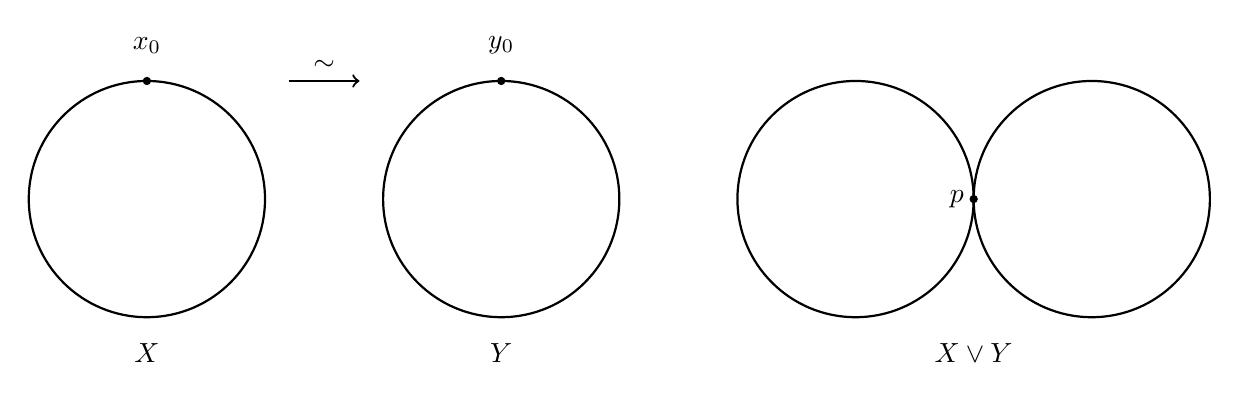
\begin{tikzpicture}[scale=1.5]
	
			% Пространство X (например, окружность)
			\draw[thick] (0, 0) circle (1);
			\fill[black] (0, 1) circle (1pt); % Выделенная точка x_0
			\node at (0, -1.3) {$X$};
			\node at (0, 1.3) {$x_0$};
	
			% Пространство Y (например, окружность)
			\draw[thick] (3, 0) circle (1);
			\fill[black] (3, 1) circle (1pt); % Выделенная точка y_0
			\node at (3, -1.3) {$Y$};
			\node at (3, 1.3) {$y_0$};
	
			% Стрелка перехода
			\draw[->, thick] (1.2, 1) -- node[above] {$\sim$} (1.8, 1);
	
			% Букет пространств
			\begin{scope}[shift={(6, 0)}]
				% Пространство X
				\draw[thick] (0, 0) circle (1);
				% Пространство Y
				\draw[thick] (2, 0) circle (1);
				% Общая точка склейки
				\fill[black] (1, 0) circle (1pt);
				\node at (1, -1.3) {$X \vee Y$};
				\node[left] at (1, 0) {$p$};
			\end{scope}
	
		\end{tikzpicture}
		
	\end{center}
	\end{example}
	
	
% \begin{example}
% 	\begin{enumerate}
% 		\item Букет
% 		\item Цилиндр 
% 		\end{enumerate}
% \end{example}
\subsection{Действие группы}


Для точки $x\in X$ множество $G(x) = \{g(x)\ |\ g\in G\}$ называют орбитой точки $x$ под действием группы $G.$
Согласно задаче (тут надо на неё послать), орбиты задают разбиение множества $X.$ \


Лемма 1 ( правильная).  Пусть $X$ - хаусдорфово пространство, $K\subset X$ - компакт, и $x\in X\setminus K.$ Тогда тогда $x$ и множество $K$ могут быть отделены непересекающимися окрестностями.\\

Док-во. Для всякой точки $k\in K$ существует окрестность $U_{k}$, замыкание которой не содержит точку $x.$ В силу компактности, множество $K$ покрывается конечным числом таких окрестностей; обозначим их
через $U_{1},\ldots, U_{N}$. Положим $W = \bigcup_{i=1}^{N} U_{i}$. Тогда $K\subset W$ и $x\notin Cl(W)$, откуда $W$ и $X\setminus Cl(W)$ и дают искомые непересекающиеся окрестности.\\



Теорема (тоже правильная версия) Пусть компактная группа $G$ действует на хаусдорфовом пространстве $X.$
Тогда пространство орбит $X/G$ хаусдорфово.

Док-во.  Орбита $G(x)$ компактна, поскольку она является образом компакта $G$ при непрерывном отображении
$G \to G\times \{x\} \to G(x).$ Если $G(x)$ и $G(y)$ - различные орбиты, то по предыдущей лемме точка $x$ имеет окрестность $U$, замыкание которой не пересекается с $G(y).$
Тогда множества $p(U)$ и $(X/G) \setminus p(U)$ задают непересекающиеся окрестности точек $G(x)$ и $G(y)$ в пространстве $X/G.$

% \begin{definition}
% 	Пусть \( G \) -- группа и \( X \) -- множество. Действием группы \( G \) на множество \( X \) называется отображение \( \cdot: G \times X \rightarrow X \), удовлетворяющее следующим свойствам:
% \begin{enumerate}
%     \item Для всех \( x \in X \) выполнено \( e \cdot x = x \), где \( e \) -- единичный элемент группы \( G \).
%     \item Для всех \( g, h \in G \) и \( x \in X \) выполнено \( (gh) \cdot x = g \cdot (h \cdot x) \), где \( gh \) -- произведение элементов группы \( G \).
% \end{enumerate}
% \end{definition}

\begin{definition}[Топологическая группа]
	\textbf{Топологическая группа} $ G $ — это множество, наделенное структурой группы и хаусдорфовое топологическое пространство, такое что выполняются следующие условия:
	\begin{enumerate}
		\item Отображение умножения $ m: G \times G \to G $, заданное формулой $ m(g_1, g_2) = g_1 g_2 $, является непрерывным.
		\[
		\begin{tikzcd}[row sep=40pt, column sep=60pt]
			G \times G \arrow{r}{m} \arrow{d}{\mathrm{id} \times \mathrm{id}} & G \\
			G \times G \arrow{ur}{m}
		\end{tikzcd}
		\]
		\item Отображение взятия обратного элемента $ i: G \to G $, заданное формулой $ i(g) = g^{-1} $, является непрерывным.
		\[
		\begin{tikzcd}[row sep=40pt, column sep=60pt]
			G \arrow{r}{i} \arrow{d}{\mathrm{id}} & G \\
			G \arrow{ur}{i}
		\end{tikzcd}
		\]
	\end{enumerate}
	\end{definition}
	Когда изучается теория групп, часто говорят, например, что группа $ U(1) $ представляет собой вращения на плоскости. Однако важно понимать, что такие утверждения подразумевают не просто саму группу, а её {действие} на некотором пространстве. Действие группы формализует, как элементы группы преобразуют точки пространства, и является ключевым инструментом для изучения симметрий.

\begin{definition}[Действие группы]
Пусть $ G $ — группа, а $ X $ — множество. \textbf{Действием группы $ G $ на множестве $ X $} называется отображение
\[
\cdot : G \times X \to X, \quad (g, x) \mapsto g \cdot x,
\]
удовлетворяющее следующим условиям:
\begin{enumerate}
    \item Для любого $ x \in X $ выполнено $ e \cdot x = x $, где $ e $ — единичный элемент группы $ G $.
    \item Для любых $ g_1, g_2 \in G $ и $ x \in X $ выполнено $ g_1 \cdot (g_2 \cdot x) = (g_1 g_2) \cdot x $.
\end{enumerate}
\end{definition}
\begin{remark}
	Действие группы позволяет связать абстрактные элементы группы с конкретными преобразованиями множества $ X $. Например, группа $ U(1) $, представляющая собой комплексные числа модуля 1, действует на плоскости $ \mathbb{C} $ через умножение, что соответствует вращениям вокруг начала координат.
	\end{remark}
	Понятие орбиты точки играет ключевую роль в изучении действий групп на множествах. Оно позволяет понять, как группа преобразует пространство, и выделить подмножества точек, связанных между собой через действие группы. Это важно в различных областях математики, таких как теория групп, топология и геометрия.

	\begin{definition}[Орбита точки]
	Пусть $ G $ — группа, действующая на топологическом пространстве $ X $. Для произвольной точки $ x \in X $ множество
	\[
	G(x) = \{g(x) \mid g \in G\}
	\]
	называется \textbf{орбитой точки $ x $} под действием группы $ G $.
	\end{definition}

	Обозначим через $ X/G $ факторпространство $ X / \sim_G $, где отношение эквивалентности $ \sim_G $ задается следующим образом:
	\[
	x \sim_G y \quad \text{тогда и только тогда, когда} \quad x = g(y) \quad \text{для некоторого } g \in G.
	\]
	Таким образом, $ X/G $ — это пространство орбит, то есть множество всех классов эквивалентности точек из $ X $ относительно действия группы $ G $.
	
	Через $ p: X \to X/G $ будем обозначать соответствующее \textit{факторотображение}, которое каждой точке $ x \in X $ сопоставляет её орбиту $ G(x) $. Формально:
	\(
	p(x) = G(x) = \{g(x) \mid g \in G\}.
	\)
	\[
\begin{tikzcd}[row sep=40pt, column sep=60pt]
    G \times X \arrow{r}{\cdot} \arrow{d}{\mathrm{pr}_2} & X \arrow{d}{p} \\
    X \arrow{r}{p} & X/G
\end{tikzcd}
\]
	
\begin{example}[Примеры действий групп]
	Рассмотрим несколько важных примеров действий групп на множествах:
	
	\begin{enumerate}
		\item \textbf{Действие группы $ \mathbb{Z} $ на себе умножением:}
		Группа целых чисел $ \mathbb{Z} $ действует на множестве целых чисел $ \mathbb{Z} $ по правилу:
		\[
		\mathbb{Z} \curvearrowright \mathbb{Z}, \quad n \cdot m = n \cdot m, \quad \forall n, m \in \mathbb{Z}.
		\]
		Это действие сохраняет структуру группы и является тривиальным примером действия группы на себе.
	
		\item \textbf{Действие группы вращений $ \mathrm{SO}(2) $ на плоскости $ \mathbb{R}^2 $:}
		Группа специальных ортогональных преобразований $ \mathrm{SO}(2) $ (вращений) действует на плоскости $ \mathbb{R}^2 $. Каждое вращение $ R_\theta \in \mathrm{SO}(2) $, задаваемое углом $ \theta $, применяется к точке $ (x, y) \in \mathbb{R}^2 $ по формуле:
		\[
		\mathrm{SO}(2) \curvearrowright \mathbb{R}^2, \quad R_\theta \cdot (x, y) = (x', y'), \quad \text{где } 
		\begin{cases}
		x' = x \cos \theta - y \sin \theta, \\
		y' = x \sin \theta + y \cos \theta.
		\end{cases}
		\]
		Это действие описывает вращение точки вокруг начала координат.
	
		\item \textbf{Действие симметрической группы $ S_n $ на множестве $ \{1, 2, \ldots, n\} $:}
		Группа перестановок $ S_n $ действует на множестве $ \{1, 2, \ldots, n\} $ следующим образом:
		\[
		S_n \curvearrowright \{1, 2, \ldots, n\}, \quad \sigma \cdot i = \sigma(i), \quad \forall \sigma \in S_n, \, i \in \{1, 2, \ldots, n\}.
		\]
		Это действие соответствует перестановке элементов множества.
	
		\item \textbf{Действие классических матричных групп на $ \mathbb{R}^n $:}
		\begin{itemize}
			\item $ \mathrm{GL}_n(\mathbb{R}) $ (общая линейная группа): Действует на $ \mathbb{R}^n $ умножением матриц на векторы:
			\[
			\mathrm{GL}_n(\mathbb{R}) \curvearrowright \mathbb{R}^n.
			\]
			\item $ \mathrm{SL}_n(\mathbb{R}) $ (специальная линейная группа): Действует аналогично $ \mathrm{GL}_n(\mathbb{R}) $, но сохраняет ориентацию пространства.
			\item $ \mathrm{O}_n(\mathbb{R}) $ (ортогональная группа): Действует на $ \mathbb{R}^n $ изометриями, сохраняющими длины векторов:
			\[
			\mathrm{O}_n(\mathbb{R}) \curvearrowright \mathbb{R}^n.
			\]
			\item $ \mathrm{SO}_n(\mathbb{R}) $ (специальная ортогональная группа): Действует как $ \mathrm{O}_n(\mathbb{R}) $, но также сохраняет ориентацию.
		\end{itemize}
	
		\item \textbf{Действие унитарных групп на $ \mathbb{C}^n $:}
		\begin{itemize}
			\item $ \mathrm{U}_n(\mathbb{C}) $ (унитарная группа): Действует на $ \mathbb{C}^n $ унитарными преобразованиями, сохраняющими эрмитово скалярное произведение:
			\[
			\mathrm{U}_n(\mathbb{C}) \curvearrowright \mathbb{C}^n.
			\]
			\item $ \mathrm{SU}_n(\mathbb{C}) $ (специальная унитарная группа): Действует аналогично $ \mathrm{U}_n(\mathbb{C}) $, но с дополнительным условием сохранения определителя равным 1.
		\end{itemize}
	
		\item \textbf{Действие симметрической группы $ S_n $ на множестве подмножеств:}
		Группа $ S_n $ также может действовать на множестве всех подмножеств множества $ \{1, 2, \ldots, n\} $, переставляя элементы каждого подмножества согласно перестановке $ \sigma \in S_n $:
		\[
		S_n \curvearrowright \mathcal{P}(\{1, 2, \ldots, n\}),
		\]
		где $ \mathcal{P}(\{1, 2, \ldots, n\}) $ — множество всех подмножеств множества $ \{1, 2, \ldots, n\} $.
	
	\end{enumerate}
	\end{example}


% У нас есть: $G$ -- топологическая группа (то есть, топологическое пространство и непрерывность операций), $X$ -- топологическое пространство и пусть $G \curvearrowright X$  -- непрерывно. Тогда $X/G = X/\sim_G \ x \sim y \Leftrightarrow x = g(y)$, где $X$ -- пространство фбит.


\begin{lemma}
	Пусть $ X $ — хаусдорфово пространство, $ K \subset X $ — компактное подмножество, и $ x \in X \setminus K $. Тогда точка $ x $ и множество $ K $ могут быть отделены непересекающимися окрестностями.
	\end{lemma}
	
\begin{proof}
Для каждой точки $ k \in K $, поскольку $ X $ является хаусдорфовым пространством, существуют непересекающиеся окрестности $ U_k $ точки $ k $ и $ V_k $ точки $ x $. Заметим, что замыкание $ \overline{U_k} $ не содержит точку $ x $, так как $ V_k \cap \overline{U_k} = \emptyset $.

Таким образом, семейство открытых множеств $ \{U_k\}_{k \in K} $ образует открытое покрытие компактного множества $ K $. В силу компактности $ K $, существует конечное подпокрытие:
\[
K \subset \bigcup_{i=1}^N U_i,
\]
где $ U_1, \ldots, U_N $ — соответствующие окрестности точек из $ K $.

Определим множество
\[
W = \bigcup_{i=1}^N U_i.
\]
Тогда $ W $ является окрестностью множества $ K $, причем $ x \notin \overline{W} $ (замыкание $ W $), так как $ x \notin \overline{U_i} $ для каждого $ i = 1, \ldots, N $.

Теперь рассмотрим множества $ W $ и $ X \setminus \overline{W} $. Эти множества являются непересекающимися окрестностями множества $ K $ и точки $ x $ соответственно:
\[
K \subset W, \quad x \in X \setminus \overline{W}, \quad W \cap (X \setminus \overline{W}) = \emptyset.
\]

Следовательно, точка $ x $ и множество $ K $ могут быть отделены непересекающимися окрестностями.
\end{proof}

\begin{theorem}[Теорема о хаусдорфовости пространства орбит]
	Пусть компактная группа $ G $ действует на хаусдорфовом пространстве $ X $. Тогда пространство орбит $ X/G $ является хаусдорфовым.
	\end{theorem}
	
	\begin{proof}
	Каждая орбита $ G(x) $ компактна, поскольку она является образом компактного множества $ G $ при непрерывном отображении:
	   \[
	   G \to G \times \{x\} \to G(x).
	   \]
	Пусть $ G(x) $ и $ G(y) $ — различные орбиты в $ X $. По предыдущей лемме точка $ x $ имеет окрестность $ U $, замыкание которой не пересекается с орбитой $ G(y) $:
	   \[
	   \overline{U} \cap G(y) = \emptyset.
	   \]
	Рассмотрим образ $ p(U) $ окрестности $ U $ при факторотображении $ p: X \to X/G $. Тогда множества $ p(U) $ и $ (X/G) \setminus p(\overline{U}) $ являются непересекающимися окрестностями точек $ G(x) $ и $ G(y) $ в пространстве $ X/G $:
	   \[
	   p(U) \cap \big((X/G) \setminus p(\overline{U})\big) = \emptyset.
	   \]
	\end{proof}

	\begin{remark}[Пример нехаусдорфова факторпространства]
		Факторпространство по действию группы может оказаться нехаусдорфовым. Рассмотрим следующий пример:
		
		Группа $ \mathrm{GL}_2(\mathbb{R}) $ действует на пространстве всех $ 2 \times 2 $-матриц $ M_{2 \times 2}(\mathbb{R}) $ следующим образом:
		\[
		\mathrm{GL}_2(\mathbb{R}) \curvearrowright M_{2 \times 2}(\mathbb{R}), \quad A \cdot X = A X A^{-1}.
		\]
		
		Рассмотрим две матрицы:
		\[
		I = \begin{pmatrix}
		1 & 0 \\
		0 & 1
		\end{pmatrix}, \quad
		T_\lambda = \begin{pmatrix}
		1 & \lambda \\
		0 & 1
		\end{pmatrix}, \quad \lambda \neq 0.
		\]
		
		Заметим, что при $ \lambda \to 0 $ матрица $ T_\lambda $ стремится к единичной матрице $ I $:
		\[
		\lim_{\lambda \to 0} T_\lambda = I.
		\]
		
		Однако орбиты этих матриц под действием группы $ \mathrm{GL}_2(\mathbb{R}) $ различны:
		\[
		\text{Орбита } I: \{A I A^{-1} \mid A \in \mathrm{GL}_2(\mathbb{R})\} = \{I\},
		\]
		\[
		\text{Орбита } T_\lambda: \{A T_\lambda A^{-1} \mid A \in \mathrm{GL}_2(\mathbb{R})\}.
		\]
		
		Несмотря на то, что $ T_\lambda \to I $ при $ \lambda \to 0 $, орбиты этих матриц не могут быть разделены непересекающимися окрестностями в факторпространстве. Это показывает, что факторпространство $ M_{2 \times 2}(\mathbb{R}) / \mathrm{GL}_2(\mathbb{R}) $ не является хаусдорфовым.
		\end{remark}






